\section{Resultados}
Nesta seção, serão debatidos os resultados obtidos por meio dos dois testes realizados. O primeiro visou analisar o tempo médio de cada algoritmo, bem como a sua variância. 
No segundo teste, por outro lado, buscou-se avaliar o comportamento dos algoritmos bolha e inserção quando submetidos a vetores com diferentes taxas de ordenação, sendo estas 1\%, 3\%, 5\%, 10\% e, por fim, 50\%. 

\subsection{Variação na quantidade de elementos}
Como comentado, os resultados comprovam o comportamento quadrático do bolha, seleção e inserção. 
Entretanto, é preciso ressaltar que, se existisse uma variação significativa nos números da lista a ser ordenada, o algoritmo de contagem apresentaria um tempo para ordenar maior, podendo ultrapassar o bolha, por exemplo.

\begin{figure}[h]
    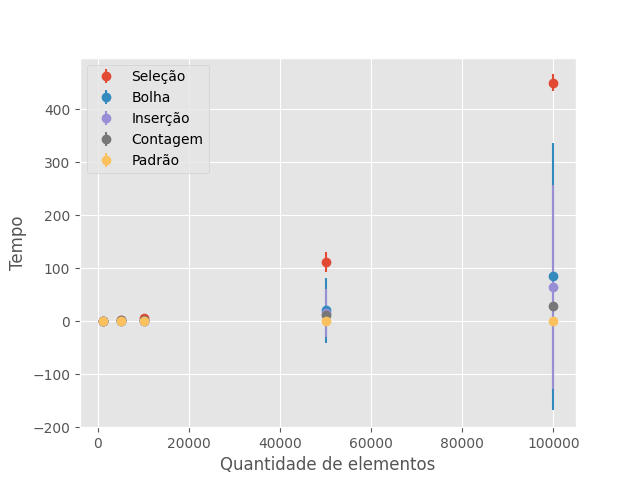
\includegraphics[width=8cm]{sizes.png}
    \caption{Gráfico elucidando o comportamento de cada algoritmo em tópico. No eixo x, há a quantidade de elementos; no eixo y, o tempo médio gasto em segundos}
    \end{figure}
\def\arraystretch{1.5}
\setlength\arrayrulewidth{0.3pt}
\begin{table}[h]
    \begin{tabular}{|l|c|F|S|S|S|S|}
    % \begin{tabular}{|l|c|c|c|c|c|c|}
    
        \hline
        \textbf{Algoritmo} & \textbf{Métrica} & \textbf{1000} & \textbf{5000} & \textbf{10000} & \textbf{50000} & \textbf{100000} \\
        \hline
        \multirow{2}{*}{\textbf{Seleção}} & \textbf{Tempo} & 0.04597 & 0.98705 & 3.88312 & 97.74410 & 389.1165 \\
        \cline{2-7}
        & $\mathbf{\sigma}$ & \num{1.38e-06} & 0.0028 & 0.0072 & 10.7685 & 6.4044 \\
        \hline
        \multirow{2}{*}{\textbf{Inserção}} & \textbf{Tempo} & 0.05796 & 1.4217 & 5.7958& 148.2008 & \num{596.8204} \\
        \cline{2-7}
        & $\mathbf{\sigma}$ & 1.68e-06 & \num{0.000222} &\num{0.001221} & 0.3690 & 1.5740 \\
        \hline
        \multirow{2}{*}{\textbf{Bolha}} & \textbf{Tempo} & 0.06942 & 1.84406 & 7.49110 & \num{194.80364} & \num{791.78906} \\
        \cline{2-7}
        & $\mathbf{\sigma}$ & \num{3.4037e-08} & \num{0.000137} & \num{0.001577} & 4.9661 & 15.7575 \\
        \hline
        \multirow{2}{*}{\textbf{Contagem}} & \textbf{Tempo} & 0.24648 & 1.21472 & 2.90298 & 14.39026 & \num{28.75249} \\
        \cline{2-7}
        & $\mathbf{\sigma}$ & \num{1.0778e-05} & \num{5.0052e-05} & \num{0.001337} & 0.0697 & 1.2251 \\
        \hline
    \end{tabular}
    \caption{Tempos de execução e desvios-padrões dos algoritmos de ordenação (em segundos) para diferentes tamanhos de lista}
    \label{tab:tempos_desvios_algoritmos_transposta}
\end{table}


O bolha, apesar de variar dependendo da taxa de ordenação, possui o maior tempo necessário para ordenar. Em seguida, o algoritmo de inserção detém o segundo maior período para organizar a sequência, e isso se dá pelo fato de que o inserção possui uma complexidade quadrática independente da posição inicial dos elementos. 

O algoritmo de seleção, como esperado, possui o melhor tempo de resposta dentre os algoritmos de comparação, tendo em vista que, além de ser mais eficiente em listas com alguns elementos ordenados, realiza menos permutações que o bolha. 

Por último, de acordo com a tabela acima, o contagem apresentou o melhor desempenho dos implementados, sendo, aproximadamente, 14 vezes mais rápido que o método de seleção. Contudo, é necessário destacar que o contagem obteve esta performance devido à faixa de números aleatórios escolhida (de 0 a 9999), pois, como analisado, o algoritmo em questão varia com os números recebidos.

Assim, percebe-se que, para listas com muitos elementos, o algoritmo contagem é o mais eficiente entre os implementados, enquanto o bolha apresentou o resultado menos satisfatório para o teste.

\newpage
\subsection{Ordenação prévia}
\begin{figure}[h]
    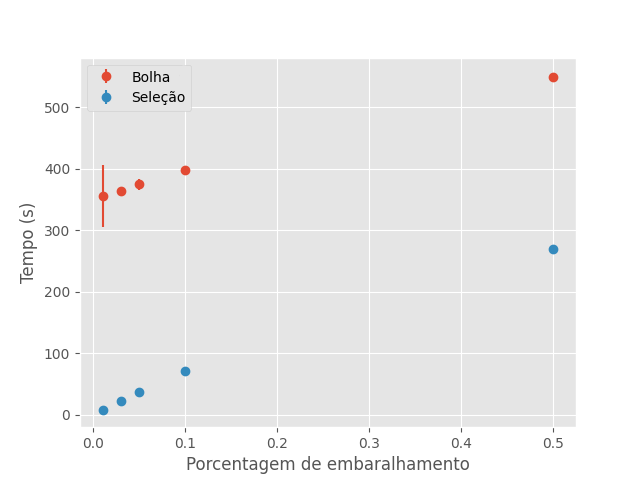
\includegraphics[width=8cm]{percentages.png}
    \caption{Gráfico ilustrando o tempo médio dos algoritmos bolha e inserção em relação à taxa de ordenação inicial dos vetores.}
\end{figure}
\def\arraystretch{1.5}
\setlength\arrayrulewidth{0.3pt}
\begin{table}[h]
    \begin{tabular}{|l|c|c|c|c|c|c|}
        \hline
        \multicolumn{2}{|l|}{\textbf{Porcentagem} }& \textbf{1\%} & \textbf{3\%} & \textbf{5\%} & \textbf{10\%} & \textbf{50\%} \\
        \hline
        \multirow{2}{*}{\textbf{Bolha}} & \textbf{Tempo (s)} & \num{356.6636} & \num{366.8301} & \num{376.2118} & \num{400.9899} & \num{545.8294} \\
        \cline{2-7}
        & \textbf{$\sigma$ (s)} & 0.5915 & 0.7173 & 0.8256 & 1.4911 & 1.4999 \\
        \hline
        \multirow{2}{*}{\textbf{Inserção}} & \textbf{Tempo (s)} & 7.4996 & 22.9234 & 37.1247 & 71.7217 & 274.1833 \\
        \cline{2-7}
        & \textbf{$\sigma$ (s)} & 0.0026 & 0.0057 & 0.0125 & 0.0198 & 0.1332 \\
        \hline
    \end{tabular}
    \caption{Tempo de execução e desvio-padrão de cada algoritmo em relação à taxa de ordenação da lista.}
    \label{tab:tempos_desvios_algoritmos_transposta}
\end{table}





Inicialmente, quando ambos os algoritmos são submetidos a uma lista já ordenada, o tempo de execução do algoritmo de seleção é razoável; o bolha, por outro lado, possui uma duração considerável para verificar que a lista já está ordenada. Adicionalmente, ao aumentar a permutação dos elementos, o bolha mantém a sua alta duração, principalmente devido à quantidade de comutações realizadas por este.

Por outro lado, o algoritmo de seleção apresentou um crescimento maior quando intensificada a desordenação da lista, uma vez que a quantidade de comutações realizadas pelo algoritmo tende a se aproximar a do bubble, ou seja, quanto mais ordenada a lista, mais eficiente o seleção é em comparação ao segundo.

Portanto, o algoritmo de seleção é mais eficiente do que o bolha, ainda que submetido a sequências com diferentes taxas de ordenação. Contudo, o seleção possui uma taxa de crescimento ligeiramente maior do que o bolha quando aumentada a porcentagem de embaralhamento.
